\documentclass[11pt, onecolumn, compsoc, letterpaper]{article}


% Usual setup packages
\usepackage{times}
\usepackage[utf8]{inputenc} % set input encoding (not needed with XeLaTeX)
\usepackage[margin=2.75cm]{geometry} % to change the page dimensions
\usepackage{graphicx} % General page control package
\usepackage[compact]{titlesec} % For compact title
\usepackage{listings} % For including source code with highlighting
\usepackage{subfiles} % For better multiple file per paper handling
\usepackage{hyperref} % For better hyper-link integration

% Packages for verbatim text blocks
\usepackage{alltt} % Package for including math in verbatim text
\usepackage{fancyvrb}

% Packages for math symbols and other mathey things
\usepackage{amsmath}
\usepackage{amsfonts}
\usepackage{amssymb}
\usepackage{mathtools}

% Packages for including pseudo-code
\usepackage{algorithmicx}
\usepackage{algorithm}
\usepackage{algpseudocode}

% Packages that handle lists
\usepackage{enumerate} % For reduced enumeration spacing
%\usepackage{enumitem} % For suppressing bullets
\usepackage{mdwlist} % Better control of lists

% Packages that handle tables, figures and other floats
\usepackage{tabularx}
\usepackage{multirow}
\usepackage{titling}
\usepackage{float} % To make floats movable
\usepackage[font=scriptsize,labelfont=bf]{caption}
\usepackage[font=scriptsize,labelfont=bf]{subcaption}
\usepackage{hhline}
\usepackage[usenames,dvipsnames]{color}
\usepackage[table]{xcolor}

% Packages for drawing graphs, FSMs, etc.
\usepackage{pgf}
\usepackage{tikz}
\usepackage{tikz-qtree}
\usetikzlibrary{shapes,arrows,calc,fit,positioning,shapes.symbols,shapes.callouts,patterns,automata}

% clean up references
\hypersetup{
    colorlinks,
    citecolor=black,
    filecolor=black,
    linkcolor=black,
    urlcolor=black
}

% smaller tab space
\lstset{
	tabsize=4
}

%%% HEADERS & FOOTERS
\usepackage{titlepic}
\usepackage{fancyhdr} % This should be set AFTER setting up the page geometry
\pagestyle{fancy} % options: empty , plain , fancy
\renewcommand{\headrulewidth}{0pt} % customise the layout...
\lhead{}\chead{}\rhead{}
\lfoot{}\cfoot{\thepage}\rfoot{}

%%% SECTION TITLE APPEARANCE
%\usepackage{sectsty}
%\allsectionsfont{\sffamily\mdseries\upshape} % (See the fntguide.pdf for font help)
% (This matches ConTeXt defaults)

%%% ToC (table of contents) APPEARANCE
%\usepackage[nottoc,notlof,notlot]{tocbibind} % Put the bibliography in the ToC
%\usepackage[titles,subfigure]{tocloft} % Alter the style of the Table of Contents
%\renewcommand{\cftsecfont}{\rmfamily\mdseries\upshape}
%\renewcommand{\cftsecpagefont}{\rmfamily\mdseries\upshape} % No bold!

% Nice Little macro for adding a comment box. Includes incrementing comment numbers.
\newcounter{comcount}
\setcounter{comcount}{0}
\newcommand{\mycomment}[1]
{
\refstepcounter{comcount}
\textcolor{red}{\textbf{\emph{\arabic{comcount}}: \small{#1}}}
}

% Math commands
\newcommand{\vnorm}[1]{\left|\left|#1\right|\right|}
\newcommand{\tab}{\hspace*{2em}}
\DeclareMathOperator*{\argminop}{arg\,min\,}
\DeclareMathOperator*{\argmaxop}{arg\,max\,}
\DeclarePairedDelimiter\ceil{\lceil}{\rceil}
\DeclarePairedDelimiter\floor{\lfloor}{\rfloor}
\newcommand{\argmin}[1]{\underset{#1}{\argminop}}
\newcommand{\argmax}[1]{\underset{#1}{\argmaxop}}
\newcommand{\D}[2]{\frac{d#1}{d#2}}
\newcommand{\PD}[2]{\frac{\partial #1}{\partial #2}}
\newcommand{\V}[1]{\mathbf{#1}}
\newcommand{\ubar}[1]{\underline{#1}}
\newcommand{\Sig}{\mathcal{S}}  % Sigmoid function
\newcommand{\Pl}{\mathcal{N}} % Player List
\newcommand{\Ta}{\mathcal{T}} % Targets/Resources
\newcommand{\We}{\mathcal{W}} % (All) Global Welfare Function

% Squeeze whitespace
\setlength{\parskip}{0pt}
\setlength{\parsep}{0pt}
\setlength{\headsep}{0pt}
\setlength{\topskip}{0pt}
\setlength{\topmargin}{0pt}
\setlength{\topsep}{0pt}
\setlength{\partopsep}{0pt}

\titlespacing{\section}{0pt}{*3}{*3}
\titlespacing{\subsection}{0pt}{*2}{*2}
\titlespacing{\subsubsection}{0pt}{*1}{*1}

\renewcommand{\arraystretch}{1.2}
\setlength{\droptitle}{-2cm}

\title{Performance Bounds on Centralized and Distributed Task Allocation with Constraints}
\author{Anshul Kanakia}
\date{}

\begin{document}
\maketitle

\begin{abstract}
Task allocation is a well studied problem in the fields of game theory, optimization, and computer science where a number of agents are assigned to a number of targets for maximum system welfare. For example, given a set of search/surveillance zones and a swarm of UAVs, this problem describes how the UAVs should be delegated to search zones so as to maximize some global welfare for the system. An extension of this problem is where each search zone require a minimum number of agents to be assigned to it to receive any payoff whatsoever. Another natural extension arises when certain agents cannot be assigned to specific search areas for a number of reasons such as fuel constraints, obstacles, environmental hazards, etc. We look at both these extensions and frame the problem of target threshold assignment with agent constraints as a communal welfare game and discuss distributed solutions to this problem.
\end{abstract}

%%%%%%%%%%%%%%%%%%%%%%%%%%%%%%%%%%%%%%%%%%%%%%%%%%%%%%%%%%%%%%%%%%%%%%%%%%%%%%%%
\section{Introduction}
The problem of task allocation (TA) is ubiquitous in different fields of research. In game theory, this problem is referred to as the Vehicle-Target Assignment problem. It is often called Task Allocation or Task Assignment in the field of robotics, specifically, swarm robotics and multi-agent systems. An equivalent problem is studied by ethologists to model division of labor in social insect colonies. In theoretical computer science there is a generalized formulation of task allocation called the Multiple Integer Knapsack Problem. While each of these formulations have provided unique perspectives and results, we believe an interdisciplinary approach is essential for truly leveraging the advantages brought forth via these different formulations of the common TA problem. As such, we use a game theory based problem formulation as well as Integer Programming (IP) from the field of optimization to present the most straightforward centralized approach for TA of multiple agents to multiple tasks with constraints. We then use results from swarm robotics to present a distributed approach to the problem while discussing certain problem simplifications and real-world issues such as incomplete system knowledge and transfer of information from one agent to another.

\mycomment{Move the related work paragraph here. Elaborate on the examples in the previous section and add a concrete example here. Use DARS reference to introduce the firefighting example and stick with it for the rest of the paper.}

We begin by setting up the TA problem using concise and well understood nomenclature from game theory. This formulation is then used to set up an 0-1 IP problem which optimizes a desired welfare function. The constraints for the IP evolve naturally out of the game theory formulation as well. A discussion situating the TA problem within the well known P-NP computational complexity model from computer science follows. Subsequently, we show that relaxing just one of the TA problem constrains results in an obvious centralized polynomial time greedy solution. Since the goal of this paper is to discuss bounds on the performance of \emph{distributed} approaches for solving TA, we compare the relaxed TA centralized algorithm with an analogous decentralized solution on a swarm of individually simple robots. We then re-introduce previously removed constraints and describe the complexities involved in designing a distributed solution of the TA problem. A theoretical comparison between centralized vs. decentralized approaches is once again afforded to us using the concepts of Price of Anarchy (PoA) and Price of Stability (PoS) from game theory. Finally, these theoretical results are backed up by simulated and real robot experiments.


%%%%%%%%%%%%%%%%%%%%%%%%%%%%%%%%%%%%%%%%%%%%%%%%%%%%%%%%%%%%%%%%%%%%%%%%%%%%%%%%
\section{Problem Setup and Example}\label{sec:setup}
The TA problem is formally defined as follows:
\begin{itemize}
	\item Agents/Players: $\Pl = \{n_1, n_2, \ldots, n_i, \ldots,n_{|\Pl|}\}$
	\item Targets: $\Ta = \{t_1, t_2, \ldots, t_j, \ldots,t_{|\Ta|}\}$
	\item Target Threshold: $K:\Ta \to \mathbb{Z}^+$\\
	The number of agents required to successfully attempt task-$t_j$ is $= K(t_j)$, which is shortened to $k_j$ for brevity.
	
	\item Agent Constraints: $C:\Pl \to \hat{\Ta} \subseteq \Ta$\\
	The set of constraints for agent-$n_i$ ($= C(n_i)$) is the subset of targets that this agent can reach. It is shortened to $c_i$ for brevity.
	\item Agent Assignment Matrix: A $|\Pl| \times |\Ta|$ matrix of 0-1 elements $x(n_i, t_j)$ or $x_{ij}$ for short, that are either $0$ if agent-$i$ is not assigned to target-$j$ or $1$ if agent-$i$ is assigned to target-$j$.
	\begin{equation}\label{eq:X}
		X = \left(\begin{array}{ccc}
			x_{11} & \ldots & x_{1|\Ta|}\\
			\vdots & \ddots & \vdots\\
			x_{|\Pl|1} & \ldots & x_{|\Pl||\Ta|}
		\end{array}\right)
	\end{equation}
	\item Target Assignments: $A:\Ta \to \hat{\Pl} \subseteq \Pl$\\
	The set of agents assigned to target-$t_j$ is $= A(t_j)$, which is shortened to $a_j$ for brevity. From~\eqref{eq:X} we can define
\begin{equation}\label{eq:aj}
	|a_j| = \sum\limits_{i = 1}^{|\Pl|} x_{ij}
\end{equation}
	\textbf{Definition:} A target is considered ``successfully assigned'' when $|a_j| \geq k_j$, i.e. the number of player's assigned to it is greater than or equal to its threshold value.\\
	\textbf{Definition:} A target is considered ``perfectly assigned'' when $|a_j| = k_j$.
	\item Target specific welfare function,
\begin{align}\label{eq:wf}
	W(t_j, |a_j|) & = \left\{
	\begin{array}{ll}
		w_j & |a_j| \geq k_j\\
		0 & o/w
	\end{array}\right.
\end{align}
	\item Global welfare function,
\begin{align}\label{eq:gwf}
	\We = \sum\limits_{j = 1}^{|\Ta|} W(t_j, |a_j|)
\end{align}
\end{itemize}
Given this problem setup our goal is to maximize the number of successful assignments of targets which in turn maximizes the global welfare while taking into account all agent constraints and target thresholds.

The following example describes a cooperative game with target thresholds and player constraints as seen in Figure \ref{fig:ex1}.
\begin{itemize}
	\item Agent: $\Pl = \{1,2,3,4\}$
	\item Targets: $t \in \Ta = \{a, b, c\}$
	\item Target thresholds: $k_a = k_b = k_c = 2$
	\item Agent constraints: $c_1 = c_3 = \{a, b\}$ and $c_2 = c_4 = \{b, c\}$
	\item Target specific welfare function: $W(t_j, |a_j|) = 1$ (if $|a_j| \geq k_j$), $0$ otherwise.
	
\end{itemize}
\begin{figure}[!htb]
	\centering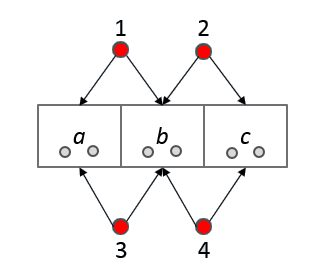
\includegraphics[width=5.5cm]{assets/ex1.png}
	\centering\caption{A cooperative game with 4 players and 3 targets. Gray pegs indicate the target's minimum threshold value while the arrows depict player assignment constraints.}\label{fig:ex1}
\end{figure}

%%%%%%%%%%%%%%%%%%%%%%%%%%%%%%%%%%%%%%%%%%%%%%%%%%%%%%%%%%%%%%%%%%%%%%%%%%%%%%%%
\section{Comparing Centralized vs. Distributed Approaches to Target Assignment}
In this section we present two approaches to solving the TA problem, one centralized and one distributed. The advantages and drawbacks of both algorithms are discussed briefly here. A more in-depth comparative discussion including performance bounds analysis follows in section~\ref{sec:disc}.

\subsection{Centralized Optimal Assignment}
Using the problem formulation from the previous section we can pose the TA optimization problem as a 0-1 IP. This means that finding an optimal assignment of agents to targets (taking constraints into account) can be achieved by using any of the many existing methods for solving IPs. This also means that the TA optimization problem exists in the realm of NP-hard problems and no polynomial time algorithm currently exists for finding such an optimal assignment. Although, as TA is a well studied problem in a number of different fields, efficient methods do exist for finding near optimal solutions. Also, given a constrained domain such as a set number of agents and relatively few targets, most existing computers can find TA solutions well within the physical movement time-frame of robots. 

The major caveat for using a centralized algorithm is that the central controller is assumed to have perfect knowledge of the operational environment and model parameters for the task being accomplished. Since this information is almost always subject to the accuracy constraints of the sensors making on-field measurements as well as the accuracy of the underlying model whose parameters are being optimized, a centralized method is not always feasible. Nonetheless, we study the effects of using a centralized controller assuming perfect system information as a baseline---being the best possible performance a multi-agent system can achieve for TA.

The IP constraints and objective to maximize are presented below using the terms defined in section~\ref{sec:setup}. 
\begin{align}\label{eq:ilp}
	\text{Maximize}\hspace{1cm} & \sum\limits_{t \in \Ta} W(t, |A(t)|) = \We\\
	\text{S. T. for all}\hspace{1cm} & i = 1\ldots|\Pl|, j = 1\ldots|\Ta|,\notag\\
	& \sum\limits_{t \in \Ta} x(n_i, t) \leq 1\notag\\
	& \sum\limits_{t \in \Ta \backslash C(n_i)} x(n_i, t) = 0\notag\\
	& 0 \leq x(n_i, t_j) \leq 1\notag
\end{align}
The first condition ensures that all agents get assigned to at most one target. The second condition accounts for each agent's target constraints $c_i$ and essentially locks in the value of $x_{ij} = 0$ for all $t_j \not\in c_i$. The final constraint makes this optimization problem a 0-1 IP since all $x_{ij}$ can only have the value $0$ or $1$. There are a number of system level quantities required for solving Eq \eqref{eq:ilp}, as shown in Table~\ref{tab:ilpquants}.

\begin{table}[!ht]
\centering\begin{tabular}{|l|p{.65\textwidth}|}
\hline
\textbf{Quantity} & \textbf{Description}\\\hline
Targets $\Ta$ & An indexed list of targets is required to match individual target thresholds and agent constraints with.\\\hline
Target Thresholds $K$ & An indexed list of team-size thresholds required to successfully attempt each task. This quantity is often extremely difficult to accurately compute. The number of robots required to complete a task can vary drastically over time due to environmental parameters, agent capabilities, and the class of tasks being performed.\\\hline
Player Constraints $C$ & An indexed list describing whether or not a particular agent can attempt a particular task. There can be a number of reasons such as an agent's on-board capabilities, path planning issues, and fuel/cost constraints that limit an agent's ability to reach or attempt a particular task. This quantity is, once again, difficult to accurately discern for a large swarm system as the internal state information for every single robot needs to either be available to the central controller or each agent must make a calculated guess as to whether or not it is capable to reaching and performing a particular task and communicate that guess back to the central controller.\\\hline 
\end{tabular}
\centering\caption{System level parameters required for solving Eq.\eqref{eq:ilp}}\label{tab:ilpquants}
\end{table}

Assuming computation and communication time between the central controller and individual agents is negligible compared to physical agent locomotion times, we can claim that this method provides a baseline definition for optimal TA. The solution, if one exists, to the optimization problem defined by Eq.~\eqref{eq:ilp} is the agent assignment matrix $X$. Of course, the optimality of the solution is conditional upon accurate value for the quantities described in Table.~\ref{tab:ilpquants}. 

\begin{figure}[!ht]
\centering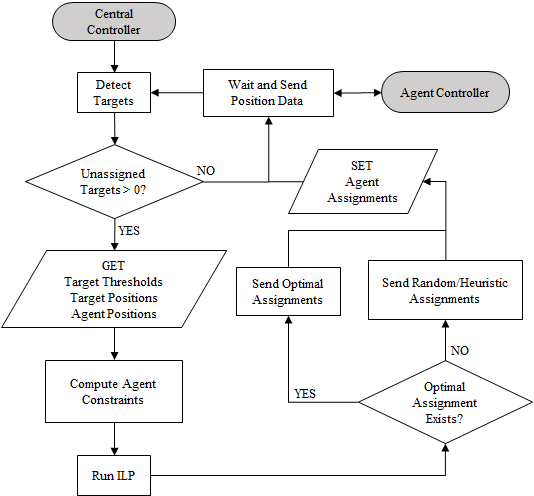
\includegraphics[width=.65\columnwidth]{assets/CentralController.png}
\centering\caption{This flowchart describes the control flow for the central controller of the centralized optimal assignment method.}\label{fig:centralcontrol}
\end{figure}

\begin{figure}[!ht]
\centering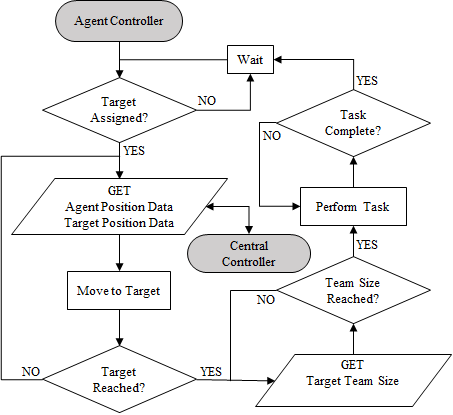
\includegraphics[width=.65\columnwidth]{assets/AgentController.png}
\centering\caption{This flowchart describes the control flow for the individual agent controller of the centralized optimal assignment method.}\label{fig:centralagentcontrol}
\end{figure}

%%%%%%%%%%%%%%%%%%%%%%%%%%%%%%%%%%%%%%%%%%%%%%%%%%%%%%%%%%%%%%%%%%%%%%%%%%%%%%%%
\subsection{Distributed Response Threshold Assignment}
Extending upon our previous work on response threshold based TA in multi-agent systems, we propose the method outlined in Fig.~\ref{fig:distcontrol} to control team-size dynamics at task sites. Each agent searches for possible collaboration targets and chooses one based on some internal heuristic, often related to minimizing path-planning complexity and energy restrictions. Since, in the distributed approach mentioned here, there is no way for an agent to discern the true magnitude of a particular target without actually inspecting it with its sensors, the choice of target to go to can be made arbitrarily. The methods used to find and select targets are not the major focus of this study and hence assumed to be readily available to each agent. Instead, we study the dynamics of estimating a target's required team size and consequently the probability of successful completion using a response threshold approach.

Each agent's probability to collaborate with the team sharing its target at a given instance of time is computed using the logistic sigmoid function and by two agent level parameters, $\tau$ and $\theta$.
\begin{equation}\label{eq:sig}
	\Sig(\tau, \theta, x) = \frac{1}{1 + e^{\theta(\tau - x)}} 
\end{equation}
$\tau$ is the average team size required to complete the given task at the target location as estimated by each individual robot using on-board sensory information and prior knowledge of the system. The $\theta$ parameter controls the allowed variance in the mean team size making it more likely for an agent to collaborate even if the measured team size, $x$, is far from the required team size, $\tau$. The relationship between $\tau$, $\theta$ and $x$ in Eq \eqref{eq:sig} imparts a continuous response threshold strategy in agents where $x$, the current team size at the target location, is the input stimulus and $\tau$ is the internal threshold for collaboration. When $x$ is $\geq \tau$ the probability to collaborate increases sharply based on the slope of $\Sig$ which, in turn, is controlled by $\theta$.



\begin{figure}[!ht]
\centering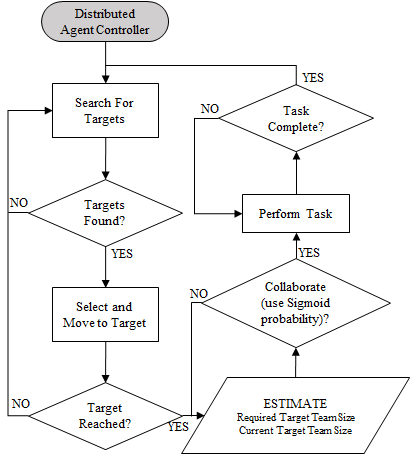
\includegraphics[width=.65\columnwidth]{assets/DistributedController.png}
\centering\caption{This flowchart describes the control flow for an indiviaul agent's controller in the de-centralized response threshold based optimal assignment method.}\label{fig:distcontrol}
\end{figure}

%%%%%%%%%%%%%%%%%%%%%%%%%%%%%%%%%%%%%%%%%%%%%%%%%%%%%%%%%%%%%%%%%%%%%%%%%%%%%%%%
\section{Experiments}
We use the Droplet swarm robot platform to perform experiments to study both the centralized and distributed approaches to TA mentioned in the previous section. 



%%%%%%%%%%%%%%%%%%%%%%%%%%%%%%%%%%%%%%%%%%%%%%%%%%%%%%%%%%%%%%%%%%%%%%%%%%%%%%%%
\section{Results}




%%%%%%%%%%%%%%%%%%%%%%%%%%%%%%%%%%%%%%%%%%%%%%%%%%%%%%%%%%%%%%%%%%%%%%%%%%%%%%%%
\section{Discussion of Performance Bounds on Centralized vs.~Distributed Approaches}\label{ref:disc}


%%%%%%%%%%%%%%%%%%%%%%%%%%%%%%%%%%%%%%%%%%%%%%%%%%%%%%%%%%%%%%%%%%%%%%%%%%%%%%%%
\section{Conclusion}


% Bibliography
% \nocite{*} % Show all Bib-entries
\bibliographystyle{plainCustom}
\bibliography{refs}
\end{document}